\chapter{Evaluating Word Vectors}\label{ch:eval}

\section{Evaluation Metrics}

We need to measure the distance between vectors to define similarity between word vectors and therefore analogies between words:

\begin{itemize}
  \item 
    \textbf{Euclidean Distance}: 
    \[
      d_\mathrm{euclid}(x,y) = \sqrt{\sum\limits_{i=1}^n(x_i - y_i)^2}
    \]

  \item 
    \textbf{Cosine Distance}
    \[
      d_\mathrm{cosine}(x,y) = 1 - \mathrm{cos}(\angle (x, y)) = 
      1 - \underbrace{\frac{\langle x,y\rangle}{\|x\|_2\|y\|_2}}_{\mathrm{Cosine\ Similarity}}
    \]
\end{itemize}

In general we could use every metric to evaluate the model. But the 
cosine similarity is more robust in terms of curse of dimensionality.

\begin{figure}[!h]
\centering
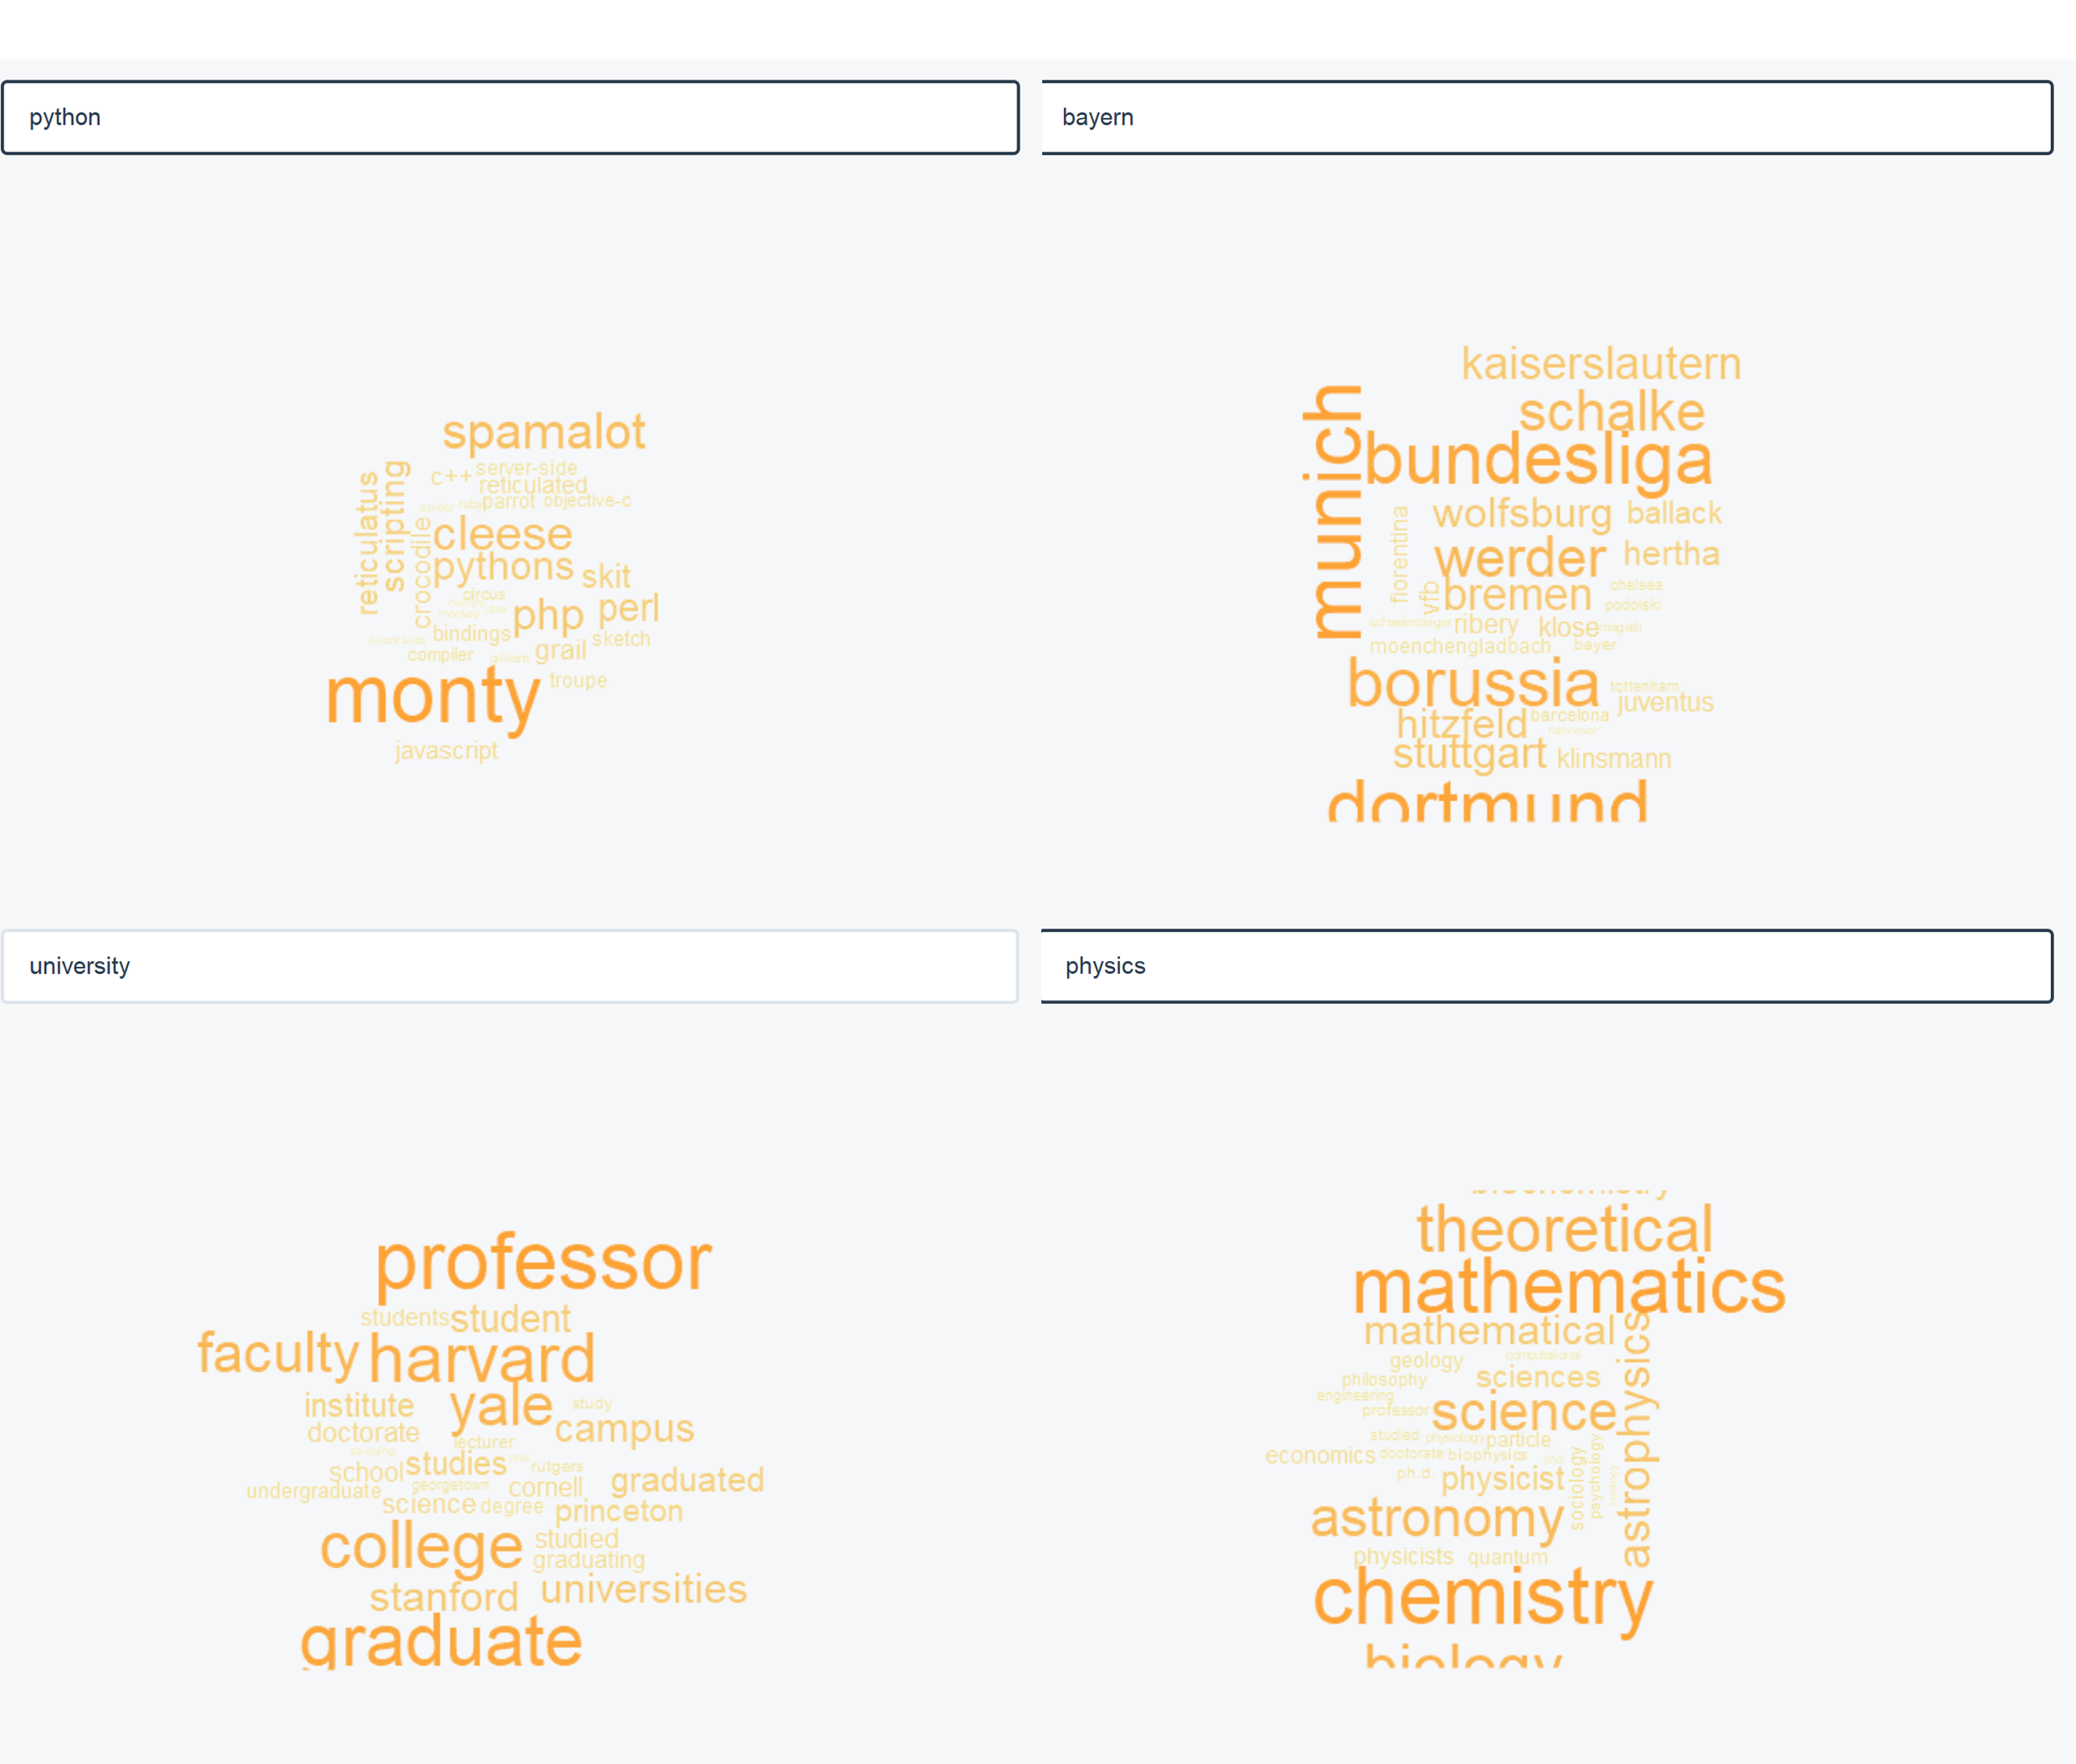
\includegraphics[scale=0.5]{images/word_clouds.png} 
\caption[Different word clouds illustrating similarities.]{Different word clouds for the words python, bayern, university and physics. The bigger the words, the smaller the cosine distance. The images are taken from an shiny application programmed for this seminar using pre trained word vectors from \cite{pennington2014glove} using the wikipedia dump (see chapter \ref{ch:data}).}
\label{fig:wc}
\end{figure}

\section{p-Norm in high Dimensions}

\cite{aggarwal2001surprising} have shown, that in high dimensions the ratio of the 
maximal norm divided by the minimal norm of $n$ points $x_1, \dots, x_n$
which are randomly drawn converges in probability to 1 for increasing
dimension $d$:
\[
\underset{{d\rightarrow\infty}}{\mathrm{p~lim}}\ \frac{\mathrm{max}_k \|x_k\|_2}{\mathrm{min}_k \|x_k\|_2} = 1
\]

$\Rightarrow$ Points are concentrated on the surface of a hyper sphere 
using the euclidean norm.

The same holds for every $p$-Norm.


{\Huge Image of p norm in high dimension}

\section{Semantic and Analogies}

One thing we now can do is to ask for semantic analogies between words. 
Something like:

\[
\mathrm{paris\ behaves\ to\ france\ like\ berlin\ to\ ?} \\
\mathrm{animal\ behaves\ to\ animals\ like\ people\ to\ ?} \\
\mathrm{i\ behaves\ to\ j\ like\ k\ to\ l} 
\]

Therefore, we have $3$ given word vectors $w_i$, $w_j$ and $w_k$. To get the 
desired fourth word $l$ we use the linearity of the word vector space:
\[
w_l \approx w_j - w_i + w_k
\]
Furthermore, we obtain $\widehat{l}$ from our model and a given metric 
$d(w_i, w_j)$ (mostly $d = d_\mathrm{cosine}$) by computing:
\[
\widehat{l} = \underset{l \in V}{\mathrm{arg~min}}\ d(w_j - w_i + w_k, w_l)
\]


\section{Questions Words File}

To evaluate trained word vectors, \cite{mikolov2013efficient} provide a word
similarity task. This task is given within a question words file which
contains about 19544 semantic analogies:

\begin{Shaded}
\begin{verbatim}
: capital-common-countries
Athens Greece Baghdad Iraq
Athens Greece Bangkok Thailand
Athens Greece Beijing China
Athens Greece Berlin Germany
Athens Greece Bern Switzerland
Athens Greece Cairo Egypt
Athens Greece Canberra Australia
Athens Greece Hanoi Vietnam
Athens Greece Havana Cuba
Athens Greece Helsinki Finland
\end{verbatim}
\end{Shaded}

\begin{center}
\begin{table}
\begin{tabular}{ l | R{2.5cm} | l }
\hline
\textbf{Category} & \textbf{Number of Test Lines} & \textbf{Example}\\
\hline\hline
capital-common-countries & 506 & Athens Greece Baghdad Iraq\\
\hline
capital-world & 4524 & Abuja Nigeria Accra Ghana\\
\hline
currency & 866 & Algeria dinar Angola kwanza\\
\hline
city-in-state & 2467 & Chicago Illinois Houston Texas\\
\hline
family & 506 & boy girl brother sister\\
\hline
gram1-adjective-to-adverb & 992 & amazing amazingly apparent apparently\\
\hline
gram2-opposite & 812 & acceptable unacceptable aware unaware\\
\hline
gram3-comparative & 1332 & bad worse big bigger\\
\hline
gram4-superlative & 1122 & bad worst big biggest\\
\hline
gram5-present-participle & 1056 & code coding dance dancing\\
\hline
gram6-nationality-adjective & 1599 & Albania Albanian Argentina Argentinean\\
\hline
gram7-past-tense & 1560 & dancing danced decreasing decreased\\
\hline
gram8-plural & 1332 & banana bananas bird birds\\
\hline
gram9-plural-verbs & 870 & decrease decreases describe describes\\
\hline
\end{tabular}
\caption{Examples for questions per category within the question word file.}
\label{tab:qwfile}
\end{table}
\end{center}

\section{Hyperparamter Tuning}

\begin{itemize}
  \item 
    Now tuning is \enquote{possible} for a given task specified in the questions words file.

  \item 
    \cite{pennington2014glove} have tuned the model and came to good values (just 
    empirical without a proof):
    \begin{itemize}
      \item $\alpha = 0.75$
      \item $x_\mathrm{max} = 100$ (does just have a weakly influence on performance)
    \end{itemize}
    
  \item 
    Note that we are dependent on this file and can just test on this file. If 
    we want to test other properties of the model we need other files.
\end{itemize}
